%!TEX root = ../prak.tex
\section{Lab 8 Digitale Ableitung und Pulsdetektion auf dem EmbSW-Roboter}
In diesem Praktikum soll eine EKG-Messung auf dem EmbSW-Roboter verarbeitet werden. Das Ziel ist, eine robuste Detektion der Herzpulse zu implementieren, damit der korrekte Puls auf der PC-Software angezeigt wird.

\medskip
\textbf{Systemübersicht}
\medskip

Die EKG-Messdaten werden vom PC einzeln über die serielle Schnittstelle auf die Hardware übertragen. Jedes Sample wird durch den Aufruf von \texttt{Ecg::processSample()} sofort verarbeitet, nachdem es vollständig empfangen wurde. Anschliessend wird es mit der detektierten Phase des Herzpulses zu einem Telegramm zusammengepackt und wieder an die PC-Software zurückgeschickt. Der Signalflussplan ist in Abbildung 1 dargestellt.

\begin{center}
  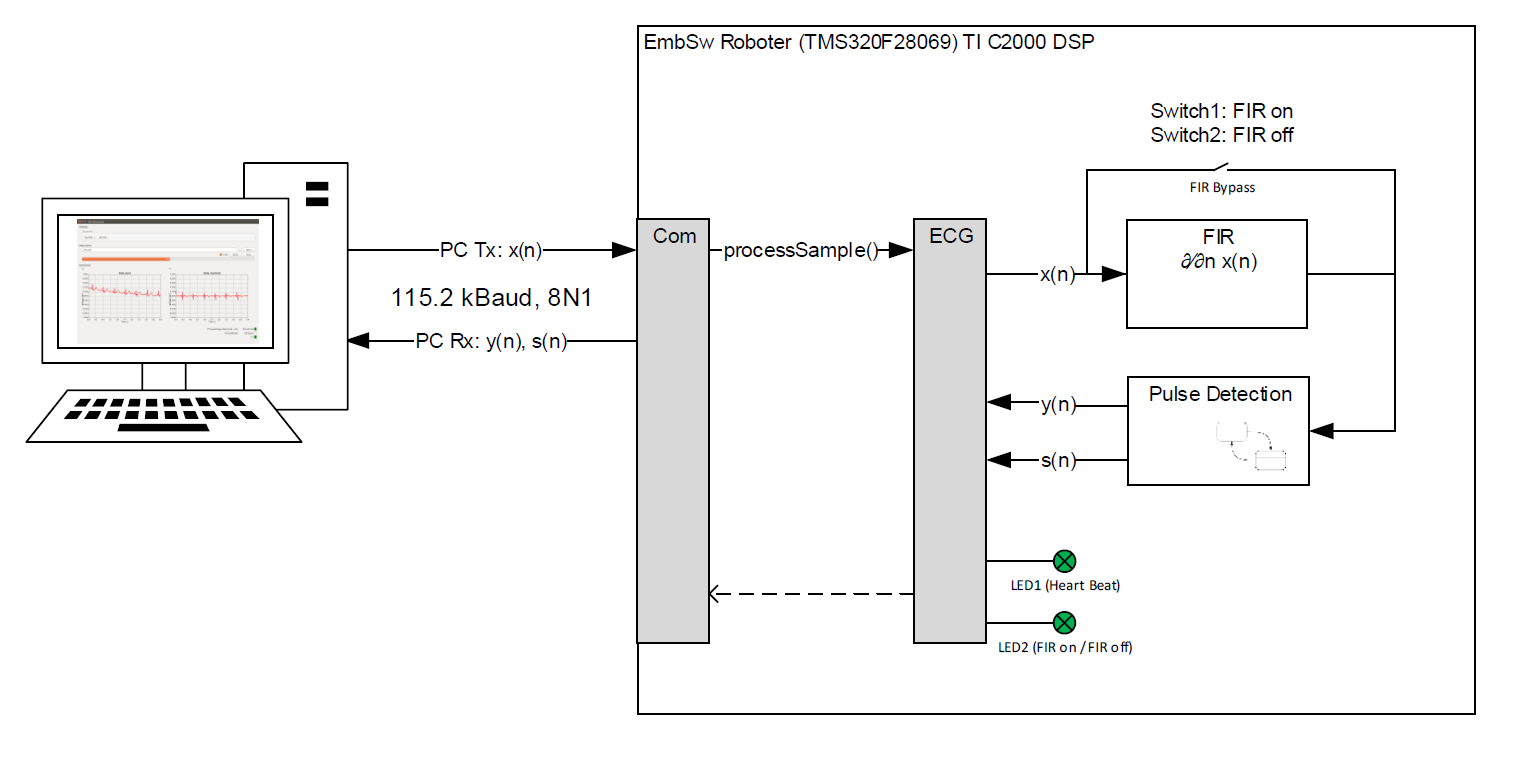
\includegraphics[width=.8\linewidth]{900-Praktika/prak08/1.PNG}
\end{center}

Die einzelnen Verarbeitungsblöcke (hier FIR und Pulse Detection) sind seriell zusammengeschaltet und können ein- bzw. ausgeschaltet werden. Mit dem Switch1 auf dem Roboter kann das FIR-Filter eingeschalten bzw. mit Switch2 wieder ausgeschalten werden.

\medskip
\textbf{Klassendiagramm der Vorgabe}

Das Vorgabeprojekt besteht aus den Klassen Ecg, Fir und PulseDetection. Zudem wird der Unit Test für diese Einheit zur Verfügung gestellt. Die Datenverarbeitung startet mit dem Aufruf von \texttt{Ecg::processSample()}. Die Klasse Ecg beinhaltet ein Array von Algorithmen, die für jedes Sample der Reihe nach abgearbeitet werden. Der neu berechnete Wert und ein detektierter Herzschlag wird schliesslich von der Funktion \texttt{Ecg::processSample()} zurück gegeben. Alle Algorithmen besitzen dieselbe Basisklasse Algorithm. In den Unterklassen muss die virtuelle Funktion \texttt{Algorithm::process(float, float\&)} überschrieben werden, um die nötige Funktion zu implementieren. Wird diese Funktion von der abgeleiteten Klasse nicht überschrieben, so hat dieser Algorithmus keinen Einfluss auf die Signalverarbeitung, da der Ausgangswert gleich dem Eingangswert gesetzt wird.
\begin{center}
  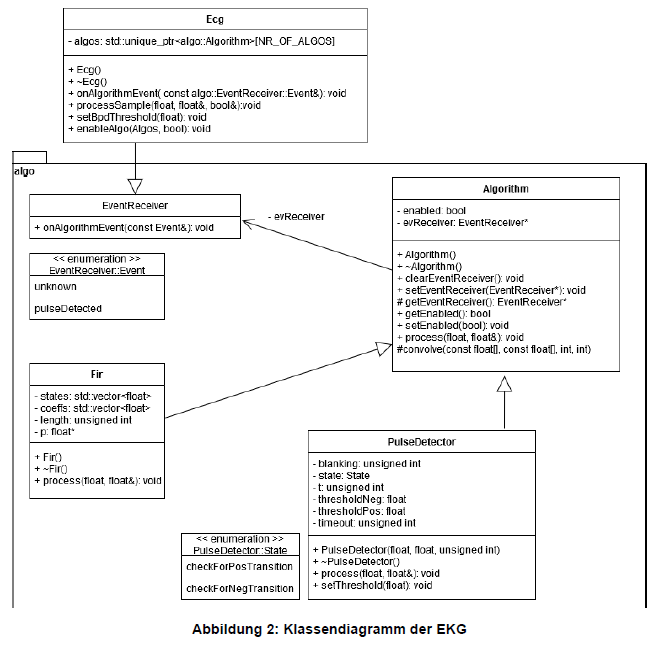
\includegraphics[width=1\linewidth]{900-Praktika/prak08/2.PNG}
\end{center}

\subsection{Aufgabe 1: Implementation des FIR-Filters}
Für eine robuste Detektion der Herzpulse soll das EKG-Signal zuerst über einen geeigneten Filter abgeleitet werden. Der Filter wird in Form eines FIR-Filters implementiert und erbt von der Klasse Algorithm. Die einfachste Variante wäre ein Filter mit den Koeffizienten $[1 \quad -1]$, was einem Differenziator entspricht. Das Ausgangssignal berechnet sich nach: $y[n] = 1\cdot x[n] – 1 \cdot x[n-1]$;
Dieses Filter reagiert stark auf die Rauschkomponente des Signals und liefert eine unbrauchbare Ableitung. Besser ist es, die Ableitung mit einer gleichzeitigen Bandpass-Filterung zu kombinieren. Eine Möglichkeit dafür ist das Savitzky-Golay-Filter (Savitzky \& Golay, 1964). Eine Analyse in MATLAB zeigt, dass eine Fensterbreite von 5 Samples und eine Ordnung von 3 eine optimale Ableitung generiert. Die resultierenden Koeffizienten sind unten abgebildet.

\texttt{static const float sgFilterCoeffs[] = \{ 0.0833, -0.6667, 0.0000, 0.6667, -0.0833 \};}

\begin{enumerate}
  \item Definieren Sie die oben erwähnten Koeffizienten in der Klasse Ecg.
  \item  Vervollständigen Sie die Methode process() der Klasse FIR indem Sie ein FIR-Filter implementieren. Mögliche Implementationen finden Sie im Buch \textit{Introduction to Signal Processing} von Sophocles J. Orfanidis, Kapitel 4.2.4 \textit{Hardware Realizations and Circular Buffers}.
  \item Testen Sie die korrekte Funktion mit dem Test Case FirTest des ECG Unit Tests. (Hinweis: Test Case PulseDetectorTest kann für diese Aufgabe auskommentiert werden.)
\end{enumerate}

\subsubsection{Lösung}

\begin{enumerate}
  \item siehe Eclipse-Projekt in ./Loesung/Ecg/, im speziellen die Klassen ./Loesung/Ecg/algo/FIR.cpp und Filterkoeffizienten in ./Loesung/Ecg/Ecg.cpp: \texttt{const float Ecg::sgFilterCoeffs[] = \{0.0833, -0.6667, 0.0, 0.6667, -0.0833\};} Die Implementation des FIR Filters ist für das bessere Verständnis sehr allgemein gehalten. Die Basis der Implementation stammt vom Buch \textit{Introduction to Signal Processing} von Sophocles J. Orfanidis, Kapitel 4.2.4 \textit{Hardware Realizations and Circular Buffers}. Für den verwendeten DSP gibt es eine Implementation eines FIR Filters von TI selbst in einer DSP-Library. Zu empfehlen sind die DSP Algorithmus-Implementationen von den Herstellern, da sie meistens sehr effizient codiert sind.
  \item Die Unit Test Cases \texttt{DisabledTest} und \texttt{FirTest} müssen fehlerfrei ausgeführt werden können. Siehe Eclipse-Projekt in ./Loesung/Ecg
\end{enumerate}

\lstinputlisting[language=C++, style=C++, multicols=2]{900-Praktika/prak08/Loesung/Ecg/Ecg.h}
\noindent\makebox[\linewidth]{\rule{\paperwidth}{0.4pt}}
\lstinputlisting[language=C++, style=C++, multicols=2]{900-Praktika/prak08/Loesung/Ecg/Ecg.cpp}
\noindent\makebox[\linewidth]{\rule{\paperwidth}{0.4pt}}
\lstinputlisting[language=C++, style=C++, multicols=2]{900-Praktika/prak08/Loesung/Ecg/testEcg.cpp}
\noindent\makebox[\linewidth]{\rule{\paperwidth}{0.4pt}}

\lstinputlisting[language=C++, style=C++, multicols=2]{900-Praktika/prak08/Loesung/Ecg/algo/EventReceiver.h}
\noindent\makebox[\linewidth]{\rule{\paperwidth}{0.4pt}}
\lstinputlisting[language=C++, style=C++, multicols=2]{900-Praktika/prak08/Loesung/Ecg/algo/FIR.h}
\noindent\makebox[\linewidth]{\rule{\paperwidth}{0.4pt}}
\lstinputlisting[language=C++, style=C++, multicols=2]{900-Praktika/prak08/Loesung/Ecg/algo/FIR.cpp}
\noindent\makebox[\linewidth]{\rule{\paperwidth}{0.4pt}}
\lstinputlisting[language=C++, style=C++, multicols=2]{900-Praktika/prak08/Loesung/Ecg/algo/PulseDetector.h}
\noindent\makebox[\linewidth]{\rule{\paperwidth}{0.4pt}}
\lstinputlisting[language=C++, style=C++, multicols=2]{900-Praktika/prak08/Loesung/Ecg/algo/PulseDetector.cpp}

\subsection{Aufgabe 2: Implementation der Pulsdetektion}
Vervollständigen Sie die Klasse \texttt{PulseDetector}. Die Methode \texttt{PulseDetector::process()} gibt das Eingangssignal wieder an den Ausgang weiter und soll nur für die Detektion der Pulse verwendet werden. Die Klasse Ecg registriert sich über \texttt{Algorithm::setEventReceiver()} und wird über diesen Callback-Mechanismus über Zustandswechsel des Pulsdetektors informiert. Sie müssen dafür sorgen, dass dieser Callback an den nötigen Stellen gefeuert wird.

In Abbildung 3 ist die Finite State Machine (FSM) für die Pulsdetektion dargestellt. Die FSM besteht aus zwei Zuständen. Im Zustand \texttt{checkForNegTransition} wird das gefilterte EKG-Signal auf negative Steigungen und in \texttt{checkForPosTransition} auf positive Steigungen überprüft. Um die Robustheit der Pulsdetektion zu erhöhen, lohnt es sich, die Zustandswechsel nicht nur über das abgeleitete Signal vorzunehmen, sondern noch Zeitkriterien einzufügen. Auf einen negativen Puls in der Ableitung muss beispielsweise unmittelbar ein positiver in der gleichen Grössenordnung folgen, damit kein DC-Offset entsteht.

\begin{center}
  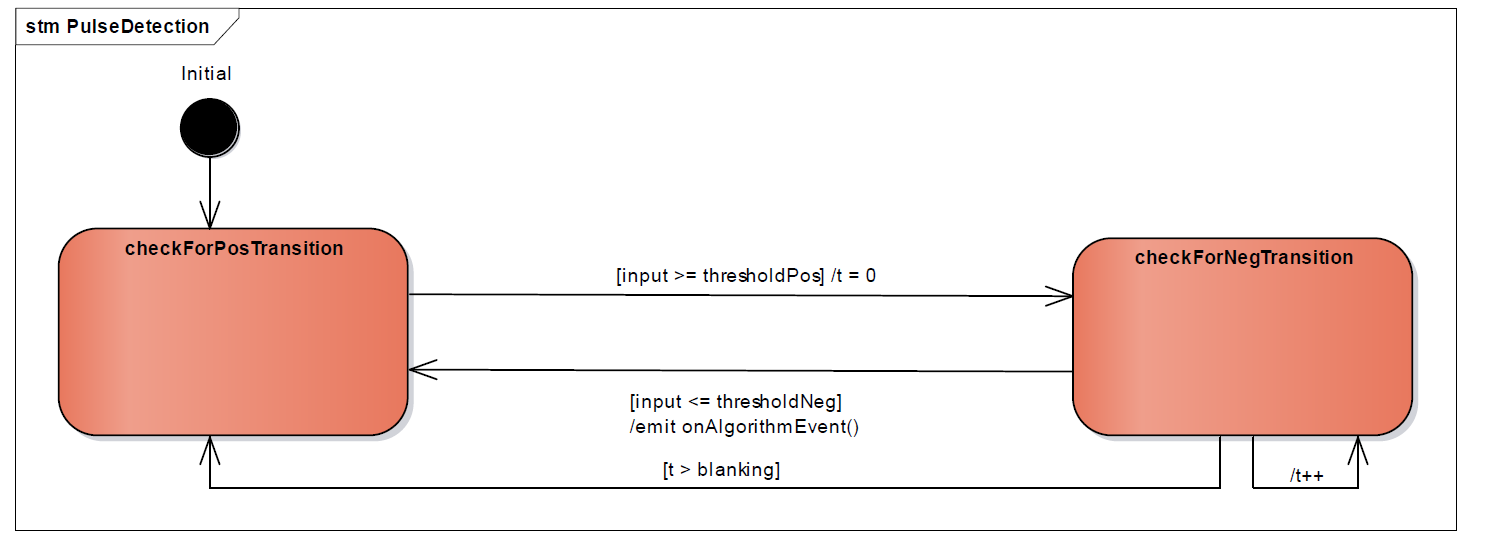
\includegraphics[width=1\linewidth]{900-Praktika/prak08/3.PNG}
\end{center}

\begin{enumerate}
  \item Implementieren Sie die Finite State Machine.
  \item Testen Sie die korrekte Funktion mit dem Test Case PulseDetectorTest des ECG Unit Tests.
\end{enumerate}

\subsubsection{Lösung}

Die Detektion basiert auf den Samples der Ableitung des EKG-Signals, einer positiven und einer negativen Detektionsschwelle (im Diagramm \textit{input, thresholdPos und thresholdNeg}). Zusätzlich existiert ein zeitliches Kriterium, damit sichergestellt ist, dass keine Störungen als Puls detektiert werden: unterschreitet die Ableitung die positive Schwelle, muss innerhalb von \textit{blanking}-Samples auch die negative Schwelle überschritten werden. Ansonsten handelt es sich mit grosser Wahrscheinlichkeit nicht um einen Herzschlag.

\begin{enumerate}
  \item siehe Klasse PulseDetector in ./Loesung/Ecg/algo/PulseDetector.h
  \item Alle Unit Test Cases müssen fehlerfrei ausgeführt werden können. Siehe Eclipse-Projekt in ./Loesung/Ecg
\end{enumerate}

\lstinputlisting[language=C++, style=C++, multicols=2]{900-Praktika/prak08/Loesung/Ecg/algo/Algorithm.h}
